\chapter{$\zeronu$ experiment status}
\section{Experimental design criteria}

As no neutrinos are emitted in a $\zeronu$ decay, the minimal observable in direct searches for $\zeronu$ decay is the total energy of the two emitted electrons.
Depending on experiment designs and purposes (detailed in Sec.~\ref{sec:zeronuexp}), individual electron energies and tracks also represent interesting observables.
The signature of a $\zeronu$ signal is an excess of events, compared to the expected background noise, in the total energy spectrum, near the $\Qbb$ released energy.
How large is this peak depends on the energy resolution of the detector.
Research for this signal involves optimising a \emph{region of interest} (ROI), also depending on the energy resolution.
The total number of events $N^{0\nu}$ occuring in the ROI and in the measurement time $t$, for a detector with an detection efficiency $\epsilon$, using a source isotope of $W$ atomic molar mass and $a$ isotopic abundance, is defined as
\begin{equation}
  N^{0\nu}=\ln(2)\frac{\mathcal{N}_{A}}{W}\left(\frac{a\epsilon M t}{\Tbeta}\right)\,\text{,}
  \label{eq:Nevents}
\end{equation}
where $\mathcal{N}_{A}$ is the Avogadro number.
If no excess of events is observed, the limit set on the $\zeronu$ decay half-life is
\begin{equation}
  T_{1/2}^{0\nu\text{,lim}}=\ln(2)\frac{\mathcal{N}_{A}}{W}\left(\frac{a\epsilon M t}{N_{\text{exc}}}\right)\,\text{,}
  \label{eq:Tlim}
\end{equation}
$N_{\text{exc}}$ being the number of $\zeronu$ events excluded at a given confidence level in the ROI.
Then, this sensitivity to the $\zeronu$ decay would depend on the number of total counts in the ROI, some of them possibly being background events:
\begin{equation}
  T_{1/2}^{0\nu\text{,lim}} \propto \left\{
  \begin{array}{ll}
    a M \epsilon t & \text{if no background is expected,} \\
    a \epsilon \sqrt{\frac{M t}{B \Delta E}} & \text{with background.}
  \end{array}
  \right.
  \label{eq:sensitivity_background}
\end{equation}
Here $B$ is the background rate usually expressed in $\Bckunit$ (when normalised to the width of the ROI, the source mass, and the observation time) and $\Delta E$ is the energy resolution.
The advantage of a background free experiment clearly comes out: the $\zeronu$ half life would increase linearly with the time of exposure $t$ (as opposed to $\sqrt t$ for an experiment with a large number of background events).
Then, it is clear that the control and the discrimination of background is of high priority for such $\zeronu$ direct search experiments.
We will discuss in Chap.~\ref{ch:detector} some important point to reduce the backgrounds for the $\zeronu$ decay detection.
Next to that, the previous expression fixes the choices that experimenters can make in designing a detector.
An ideal isotope would have a high natural abundance and would be deployed with the higest mass possible in a detector with a high detection efficiency, a good energy resolution (small $\Delta E$) under low-background conditions (small $B$).
Of all the $35$ isotopes capable of disintegrating through $\twonu$, none meets all the previous conditions.
Expermimenters will then have to find compromises, which are at the origin of the different detection strategies.
Detector can ether use an active or passive source.
In the first case, the source is also the detection medium (detector technologies detailed in Sec.~\ref{subsec:semiconductors},~\ref{subsec:bolometers} and~\ref{subsec:scintillators}).
In the second case, the source is decoupled from the detection part of the experiment (see Sec.~\ref{subsec:TPC} and~\ref{subsec:trackocalo}).
In the next section, we provide a review of the current and future experiments that aim to discover the neutrinoless double beta decay.

\subsection{Aspects of the nuclear matrix elements}
\label{subsec:matrix_element}
\subsection{Quenching}
\label{subsec:quenching}

\section{$\zeronu$ direct search experiments}
\label{sec:zeronuexp}
\subsection{Semiconductors}
\label{subsec:semiconductors}
Various semiconductor technologies are employed in the detection of $\zeronu$ decay.
The $^{76}$Ge $\beta\beta$ emitter ($\Qbb=2039$ keV) is historically important as it has been adopted since the 1960s in $\zeronu$ decay searches, acting as active source, which enhances the detection efficiency.
$^{76}$Ge-enriched high purity Germanium detectors (HPGe) offer both high energy resolution and extremely high radiopurity (as impurities are removed in the crystal growing process).
These characteristics allow, once external background contribution is minimised, to reach high sensitivity on $\zeronu$ decay, which makes this category of detectors one of the most promising for ton-scale experiments.
Since the last generation (IGEX and Heidelberg-Moscow), HPGe detectors had been improved to reach an ultra low background rate, making way for the current generation of $\zeronu$ detectors -- GERDA, MAJORANA demonstrator and LEGEND.\\

The \textbf{GERDA} experiment (GERmanium Detector Array) is located at the Laboratori Nazionali del Gran Sasso (LNGS), Italy.
GERDA phase I was running from $2011$ to $2013$ with $17.8$ kg of enriched active source detectors from the HEIDELBERG-MOSCOW and IGEX experiments.
Its first aim was to put to the test the controversial result of HEIDELBERG-MOSCOW experiment given in $2001$, announcing the first evidence for $\zeronu$ signal at a $4.2\sigma$ confidence level.
With an exposure of $21.6$ kg.y, the absence of signal in the GERDA-I experiment refuted the previous result, setting a limit $\Tbeta>2.1\, 10^{25}$ y.
Since $2015$, the GERDA experiment is in the second phase (see Fig.~\ref{fig:GERDA}), with a total of $35.8$ kg enriched detectors, $20$ kg of which is Broad Energy Germanium (BEGe) detectors that have been deployed for GERDA-II, providing a better energy resolution and pulse shape discrimination.
The active source is deployed inside a liquid Argon (LAr) augmented with light sensors, acting as an active external shield as well as a cooling down system.
The total is surrounded by a water tank.
The aim is to reach a $10^{26}$ y sensitivity with $100$ kg.y exposure, and a background rate less than $10^{-3}$ $\Bckunit$.
The underground laboratory of INFN provides $3500$ m water equivalent to reduce the external cosmic background.
In $2019$, a combined analysis for GERDA phases I and II has resulted in a half-life limit of $\Tbeta>0.9\, 10^{26}$ y ($90$\% C.L., sensitivity assuming no signal is $1.1\, 10^{26}$), corresponding to an effective neutrino mass of $\mbb<0.07\text{-}0.16$ eV ($90$\% C.L.)\footnote{This result depends on the nuclear matrix elements used for the calculations. See Sec.~\ref{subsec:matrix_element}.}.


\begin{center}
  \begin{table}
    \begin{tabular}{l  c  c  c  c}
      \hline \hline
      Experiment &  Isotope  & M (kmol)&$\Tbeta$ ($90$ \% C.L.)&  $\mbb$ (meV)\\
      \hline
      GERDA~\cite{art:GERDA2019}        & $^{76}Ge$  & $0.41$  & $9\,10^{25}$          & $104-228$    \\
      MAJORANA~\cite{art:majorana2019}  & $^{76}$Ge  & $0.34$  & $2.7\,10^{25}$        & $157-346$    \\
      CUPID-$0$~\cite{art:CUPID2018}    & $^{82}$Se  & $0.063$ & $0.24\,10^{25}$       & $394-810$    \\
      CUORE~\cite{art:CUORE2018}        & $^{130}$Te & $1.59$  & $1.5\,10^{25}$        & $162-757$    \\
      EXO-$200$~\cite{art:EXO2018}      & $^{136}$Xe & $1.04$  & $1.8\,10^{25}$        & $93-287$     \\
      KamLAND-Zen~\cite{art:KamLAND2016}& $^{136}$Xe & $2.52$  & $10.7\,10^{25}$       & $76-234$     \\
      \hline \hline
    \end{tabular}
  \end{table}
\end{center}


\begin{figure}
  \centering
  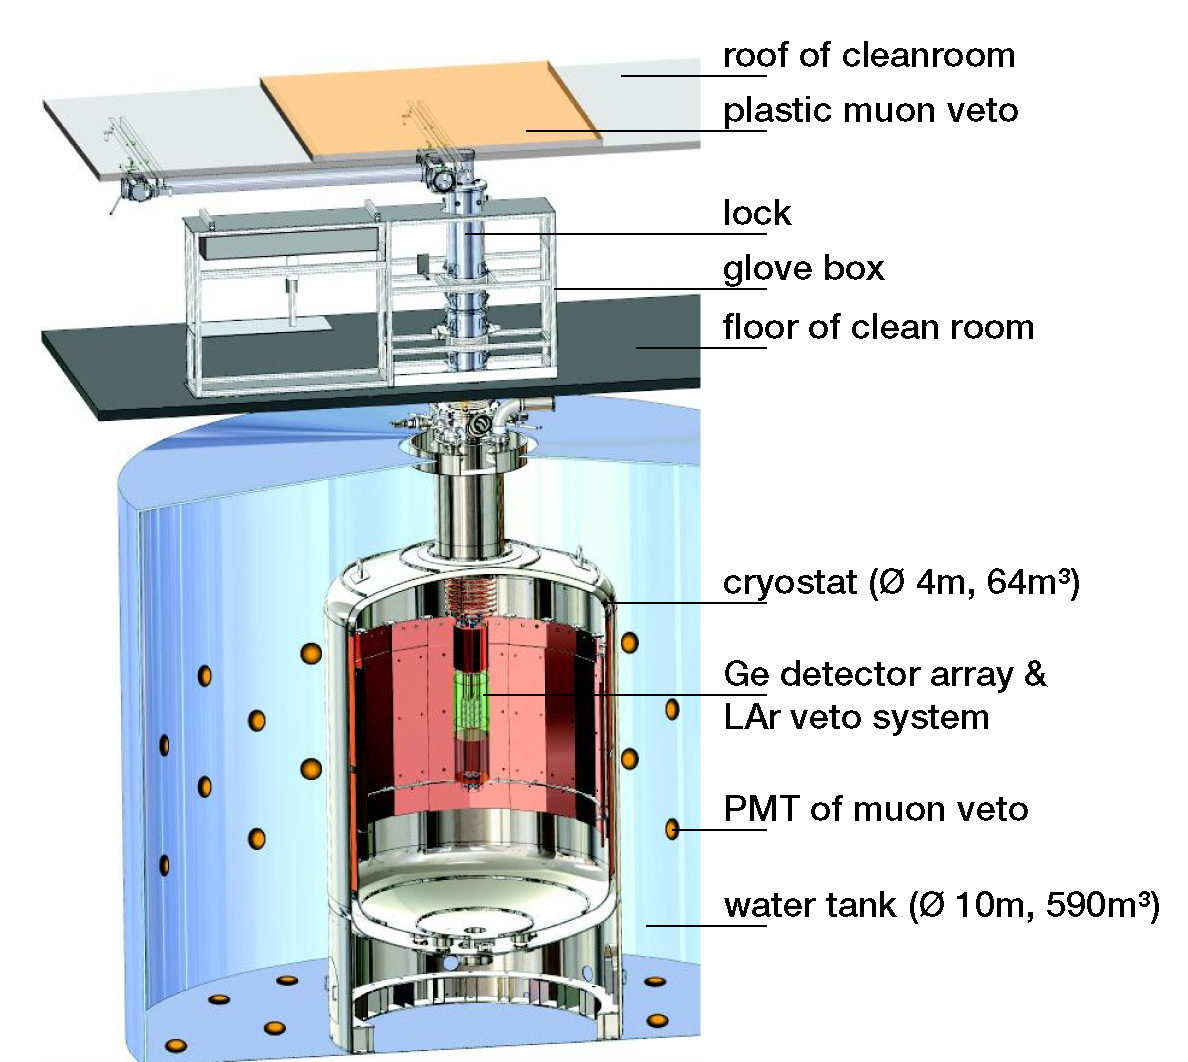
\includegraphics[width=10cm]{0nubbexperiments/fig_0nubbexperiments/GERDA.png}
  \caption{}
  \label{fig:GERDA}
\end{figure}


\textbf{MAJORANA demonstrator}

\textbf{LEGEND}
\subsection{Bolometers}
\label{subsec:bolometers}

Bolometers are high energy resolution and high detection efficiency calorimeters operating at low temperatures ($\simeq 10-20$ mK).
This type of detector is particularly suitable for $\zeronu$ searches, with the possibility of building large-scale experiments.

\textbf{CUORE}\\
\textbf{CUPID}\\
\textbf{AMoRE}
\subsection{Time projection chambers}
\label{subsec:TPC}

Time Projection Chambers (TPC) detectors use a medium producing two ways to measure the electron energies: a \emph{scintillation} (ultra-violet light) prompt signal, and a \emph{ionisation} delayed signal.
When a particle crosses the detector, a scintillation light is emitted, the energy of the scintillation peak depending on the medium.
Scintillation photons, travelling at speed of light in the medium, are detected by photosensors, giving the \emph{zero-time} of the event.
The crossing particle ionises the medium all along its way, creating electrons drifting to a collection system (an electric field is applied between cathode and anode), allowing the precise measurement of the electron production location in a 2D plane.
The drift time measurement gives access to the third coordinate of the interaction point.
Therefore, combining the two consecutive signals allows precise position and energy reconstruction.
An discriminating observable is the ionisation-to-scintillation ratio (see Fig.~\ref{fig:ratio_EXO-200}) as it provides particle discrimination between $\alpha$ particles (low ratio) and $\gamma$ radiations and $\beta$ particles (high ratio).
For $\zeronu$ searches, $^{136}$Xe-enriched isotope in liquid phase is used, offering a maximal source density (more compact detecors) and a good position resolution.
Unfortunately, the energy resolution is worse than that of the gas-phase TPCs detectors\footnote{Two-phase liquid-Xenon detectors are developed for Dark Matter searches and could be exploited for $\zeronu$ direct searches with the DARWIN project.}.
Noble elements are natural radiation detectors, avoiding the need for excess materials that could generate extra radioactive backgrounds.
$^{136}$Xe-enriched is the only noble element capable to $\twonu$ decay, with $\Qbb=2457.8$ keV.
This isotope has a relatively high natural abundance ($9$\%), can be enriched to highly pure concentrations, and does not have other long-lived radioactive isotopes, making it interesting for large-scale TPCs $\zeronu$ experiments.\\

The \textbf{EXO-$200$} experiment is a prototype of the Enriched Xenon Observatory (EXO) project, currently operating in a room under an overburden of $1624$ m.w.e, at the Waste Isolation Pilot Plant (WIPP), USA.
The detector is shaped as a cylinder, with two back-to-back cylindrical TPCs.
A high negative voltage grid cathode helds at the mid plane of the detector ($40$ cm diameter), and two anodes are located on both sides, at ground potential.
A cross-section of the detector is displayed in Fig.~\ref{fig:EXO-200}.
With $110$ kg of enriched $^{136}$Xe in liquid phase (the detector is held at $167$ K in a cryongenic bath), the phase I of this TPC detector has measured for the first time the Xenon $\twonu$ decay with $\Tbeta=2.165\times 10^{21}$ y.
Between phase I and IIa, the detector was upgraded with improved low-noise electronics, a Radon suppression system, and the impurities contents of the Xenon were reduced by a factor ten.
The current detector performance shows an energy resolution of $2.90$\% (FWHM) at the decay $Q$-value and a background rate of $(1.6)\times 10^{-3}\Bckunit$.
EXO-$200$ phase IIa data placed a new limit of $\Tbeta>1.8\times 10^{25}$ y ($90$\% C.L.).
The final analysis of data is in progress.


\begin{figure}
  \centering
  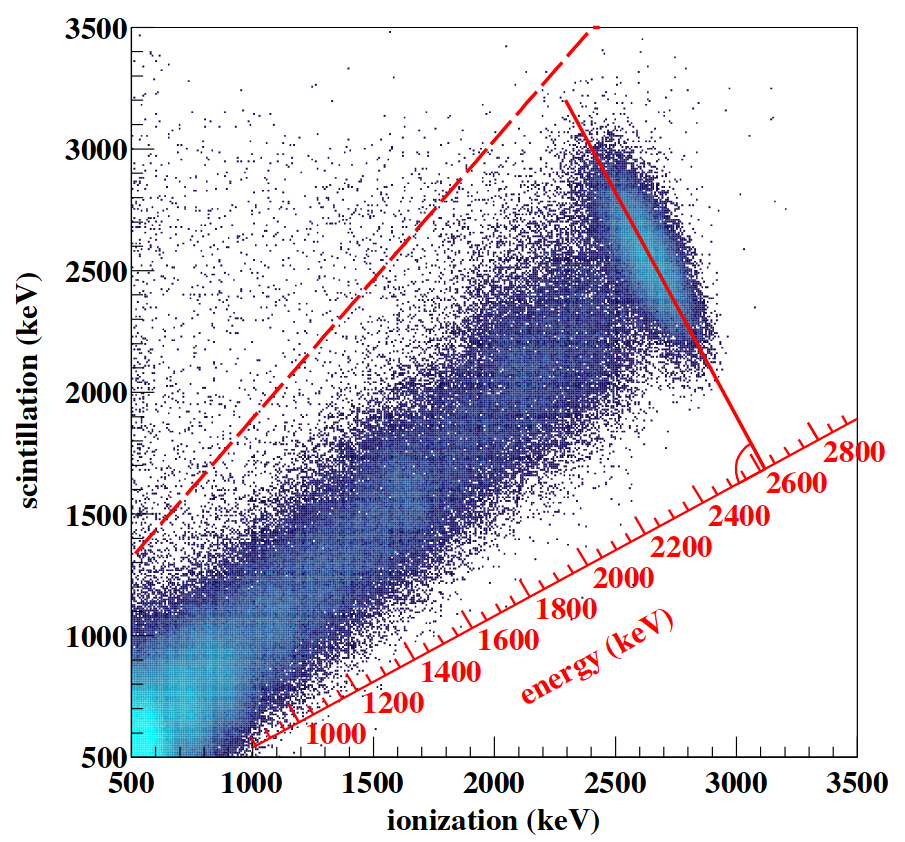
\includegraphics[width=8cm]{0nubbexperiments/fig_0nubbexperiments/ionisation-to-scintillation_EXO-200.png}
  \caption{}
  \label{fig:ratio_EXO-200}
\end{figure}

\begin{figure}
  \centering
  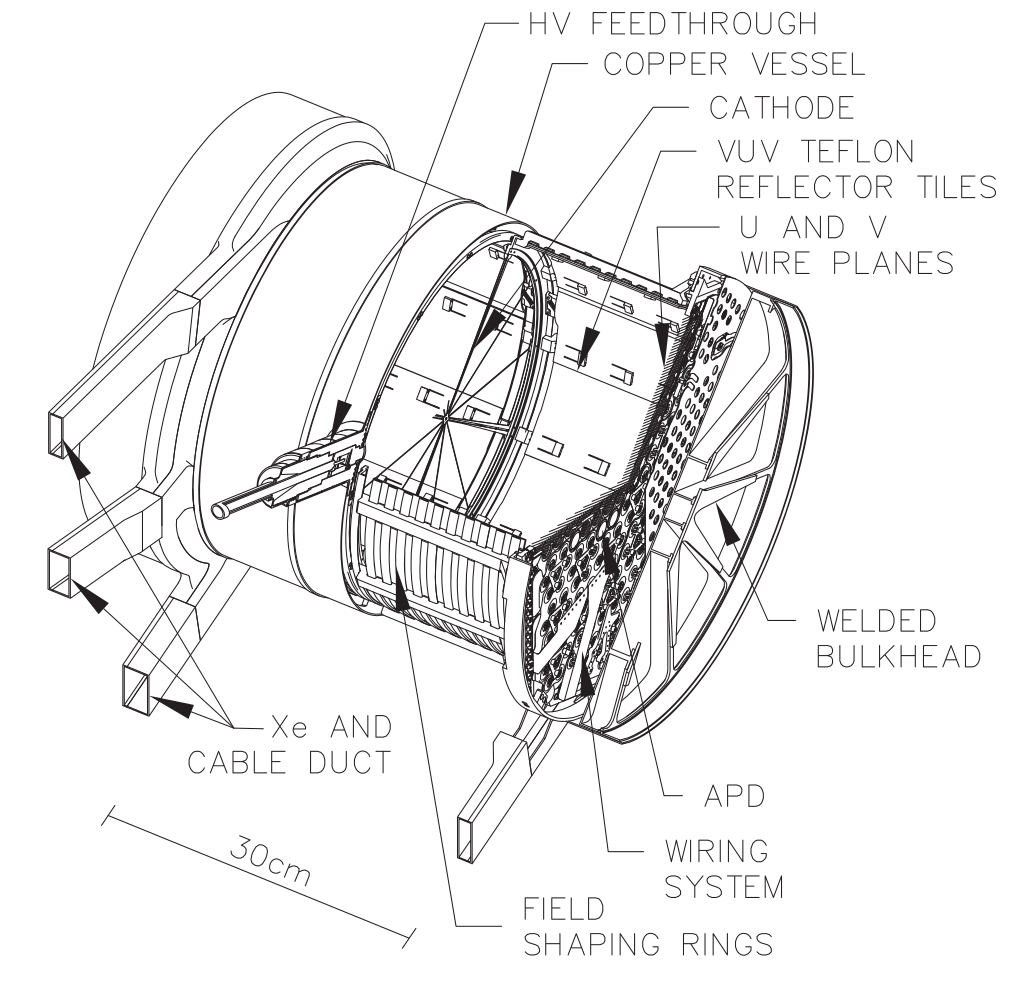
\includegraphics[width=8cm]{0nubbexperiments/fig_0nubbexperiments/EXO-200.png}
  \caption{}
  \label{fig:EXO-200}
\end{figure}

\textbf{nEXO}\\
\textbf{NEXT}\\
\textbf{PandaX-III}
\subsection{Scintillators}
\label{subsec:scintillators}
\textbf{KamLAND-ZEN and KamLAND2-ZEN}\\
\textbf{ZICOS}\\
\textbf{CANDLES}
\subsection{Tracking calorimeters}
\label{subsec:trackocalo}
Tracking calorimeters technology, instead of using a \emph{source-as-detector}, employ a passive source shaped as thin source foils of enriched $\beta\beta$ emitters.
Sources are placed at the detector centre, surrounded by two trackers allowing for particle identification (between electrons, positrons, $\gamma$ and $\alpha$ particles) and vertex reconstruction to improve the background rejection.
The whole is sandwiched between calorimeters enabling individual particle energy reconstruction.
In case of a discovery, this passive source tracking calorimeter technology provides topological information on angular emissions of the two electrons from $\beta\beta$ decay, making possible to distinguish between underlying mechanisms for $\zeronu$ decay (see Sec.~\ref{subsec:nu_mass_nature}).\\

The \textbf{SuperNEMO} experiment is a next-generation of detector, inheriting the lineage of the NEMO (Neutrino Ettore Majorana Observatory) experiments, which successfully studied multiple isotopes as enriched Molybdenum $^{100}$Mo.
